
Execution+mypy repair substantially outperforms execution-only repair on HumanEval+ (+8.94pp pass@1), consistently across three seeds. The improvement is not explained by type-targeted correction. The Z3 extension provides no additional benefit at the current counterexample activation rate.

\subsubsection{RQ1: Mypy Signal Existence (h-e1)}

On HumanEval+ (100 problems, 1 seed, 30 failing solutions sampled), \textbf{70\% of failing solutions} (21/30) have at least one mypy-detectable error --- substantially exceeding the 10\% existence gate. On MBPP+ (100 problems, 1 seed, 21 failing solutions sampled), \textbf{0\% of failing solutions} (0/21) have mypy errors.

All 100\% of detected mypy errors in HumanEval+ are in the \texttt{name-defined} category --- hallucinated function or variable name references. Error categories \texttt{arg-type}, \texttt{return-value}, and \texttt{attr-defined} are absent. This indicates that GPT-4o-mini's primary mypy-detectable failure mode on HumanEval+ is hallucinating undefined identifiers rather than producing type-incorrect expressions.

Gate h-e1 (MUST\_WORK): \textbf{PASS} --- HumanEval+ fraction 70\% exceeds the 10\% threshold; MBPP+ fraction 0\% does not, establishing the benchmark divergence.

\begin{figure}[htbp]
\centering
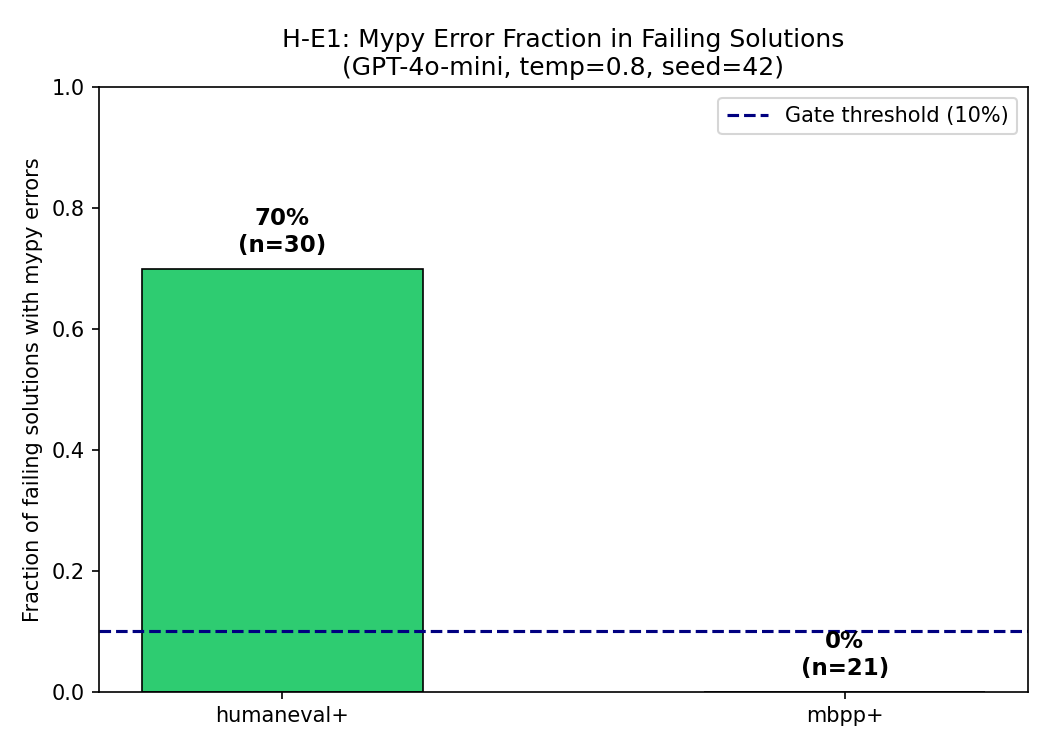
\includegraphics[width=\columnwidth]{figures/fig1_mypy_fraction_by_benchmark.png}
\caption{Fraction of failing solutions with mypy-detectable errors on HumanEval+ and MBPP+}
\label{fig:fig1_mypy_fraction_by_benchmark}
\end{figure}

\textit{Figure 1: Fraction of GPT-4o-mini failing solutions with mypy-detectable errors on HumanEval+ (70\%) and MBPP+ (0\%). Gate threshold at 10\%.}

\begin{figure}[htbp]
\centering
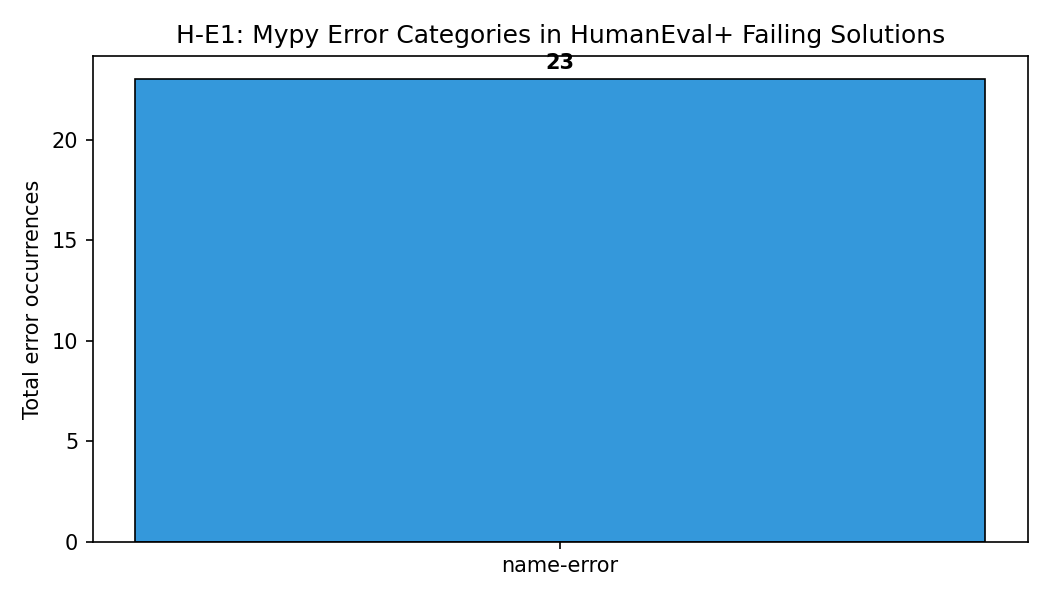
\includegraphics[width=\columnwidth]{figures/fig2_error_category_breakdown.png}
\caption{Mypy error category breakdown in HumanEval+ failing solutions}
\label{fig:fig2_error_category_breakdown}
\end{figure}

\textit{Figure 2: Mypy error category counts in HumanEval+ failing solutions. All 23 error occurrences across 21 failing solutions are in the \texttt{name-defined} category.}

\subsubsection{RQ2: LLM Consumption of mypy Feedback (h-m1)}

Among 20 HumanEval+ problems with at least one initial mypy error under Condition B (full 164-problem run, seed=42), mean mypy errors follow a near-perfect monotonic decrease: \textbf{1.55 ($\pm 0.687)$ at round 1, 0.00 ($\pm 0.000)$ by round 2}, remaining at 0.00 through rounds 3--5. No backsliding is observed.

Spearman $\rho = -0.707$ (p=0.182). The p-value of 0.182 reflects the mathematical limitation of Spearman testing with n=5 data points --- statistical significance at p<0.05 is unachievable with n=5 for this near-step-function trajectory and does not indicate a weak effect. The effect is unambiguous: all 20 eligible problems eliminate mypy errors within a single repair round.

MBPP+ contributes no data: 0/378 MBPP+ problems have initial mypy errors (consistent with RQ1), confirming that the monotonic reduction analysis applies to HumanEval+ only.

Gate h-m1 (MUST\_WORK): \textbf{PASS} --- Spearman $\rho = -0.707$ < 0; round 5 mean (0.00) < round 1 mean (1.55); mechanism activated.

\begin{figure}[htbp]
\centering
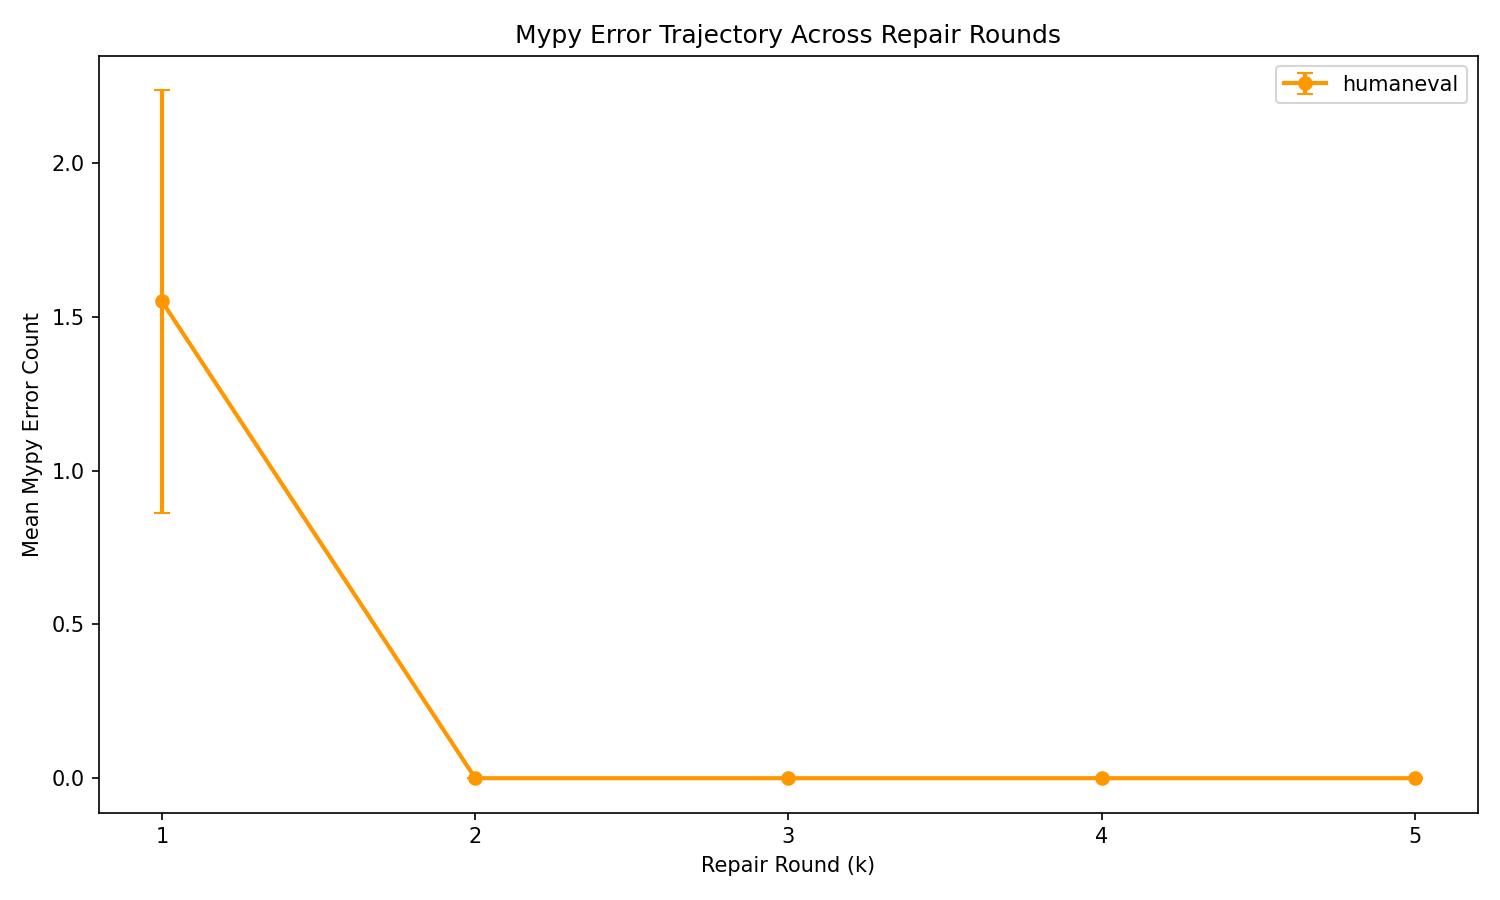
\includegraphics[width=\columnwidth]{figures/error_trajectory.png}
\caption{Mean mypy error count by repair round}
\label{fig:error_trajectory}
\end{figure}

\textit{Figure 3: Mean mypy error count ($\pm std)$ by repair round for n=20 HumanEval+ problems with at least one initial mypy error under Condition B. Errors drop from 1.55 at round 1 to 0.00 by round 2 and remain at 0.00 through round 5. Spearman $\rho = -0.707$.}

\begin{figure}[htbp]
\centering
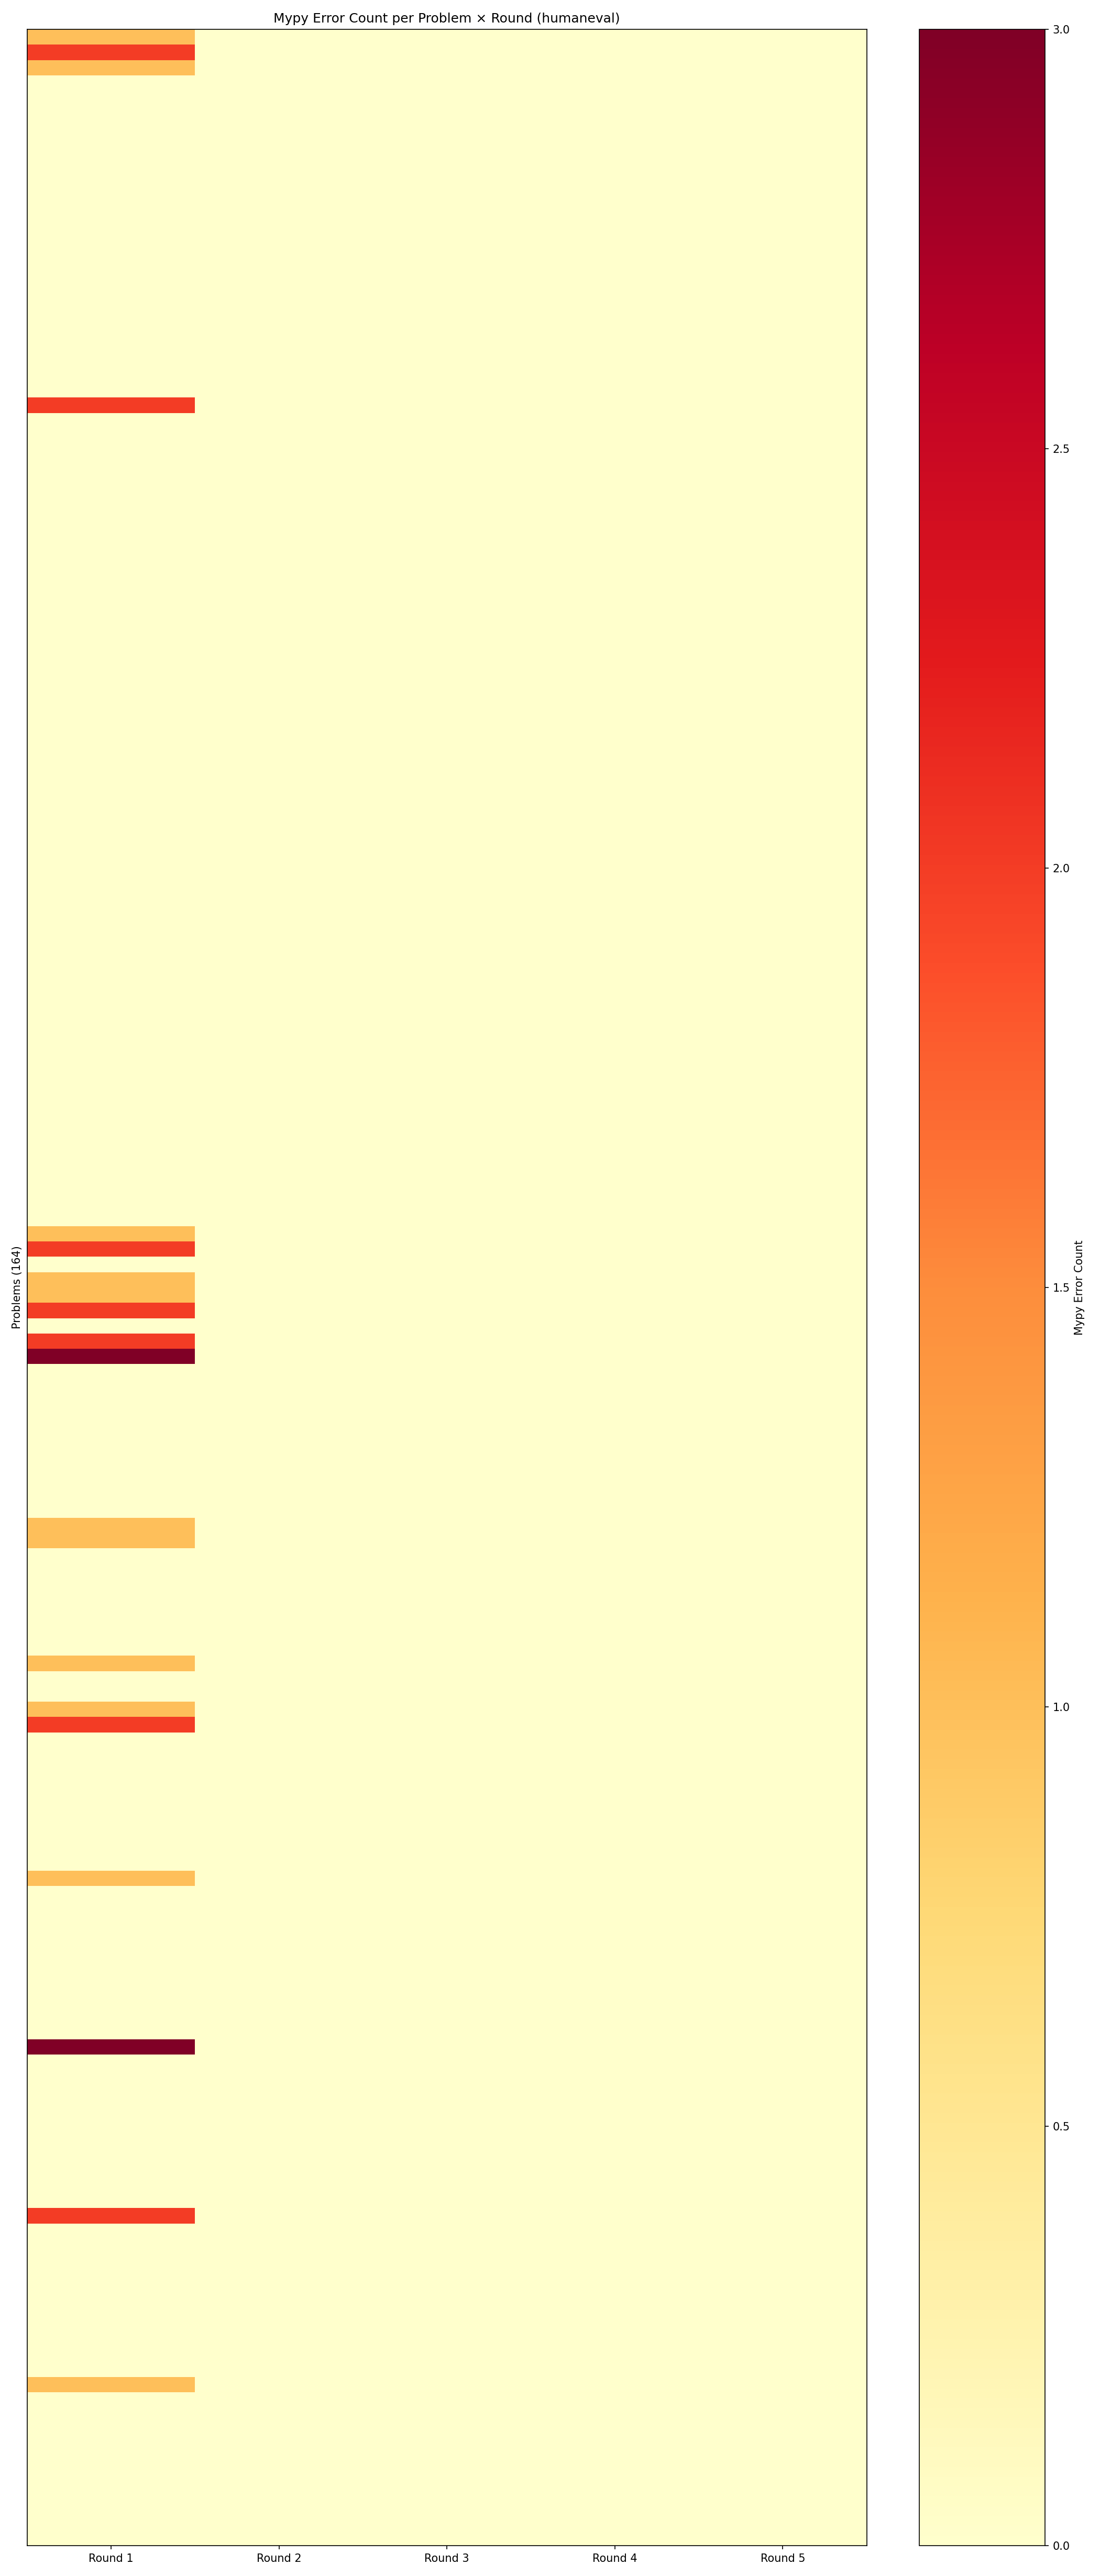
\includegraphics[width=\columnwidth]{figures/heatmap_humaneval.png}
\caption{Per-problem heatmap of mypy errors by repair round}
\label{fig:heatmap_humaneval}
\end{figure}

\textit{Figure 4: Per-problem $\times$ repair round heatmap of mypy error counts for eligible HumanEval+ problems.}

\subsubsection{RQ3: Type-Specificity of Improvement (h-m2)}

\textbf{Table 1:} Repair rates by problem type and condition (HumanEval+, seed=42, k=5 rounds).

\begin{table*}[htbp]
\centering
\resizebox{\dimexpr 2\columnwidth+\columnsep\relax}{!}{%
\begin{tabular}{lllll}
\toprule
Problem type & n & Condition A (exec-only) & Condition B (exec+mypy) & Delta ($B-A)$ \\
\midrule
Type-error & 22 & 90.9\% & 90.9\% & **0.000** \\
Non-type-error & 142 & 83.8\% & 84.4\% & **+0.006** \\
\bottomrule
\end{tabular}
}
\end{table*}

Type-specificity differential = delta\_type $-$ delta\_non = 0.000 - 0.006 = \textbf{$-0.006$}.

Both conditions achieve exactly 90.9\% repair rate on type-error problems (20/22 repaired under both conditions). The type-specificity mechanism is not supported: execution-only repair is as effective as execution+mypy repair for type-error problems at k=5.

Two confounds are consistent with this null result: (1) a ceiling effect --- type-error problems may be structurally easier, reaching near-ceiling (90.9\%) under execution-only repair before mypy can show differential benefit; (2) k=5 saturation --- differential signal may appear at early rounds (k=1..2) before it washes out. The n=22 type-error problem count also limits statistical power.

Gate h-m2 (SHOULD\_WORK): \textbf{FAIL} --- differential = $-0.006 \leq$ 0; route to EXPLORE; limitation recorded.

\begin{figure}[htbp]
\centering
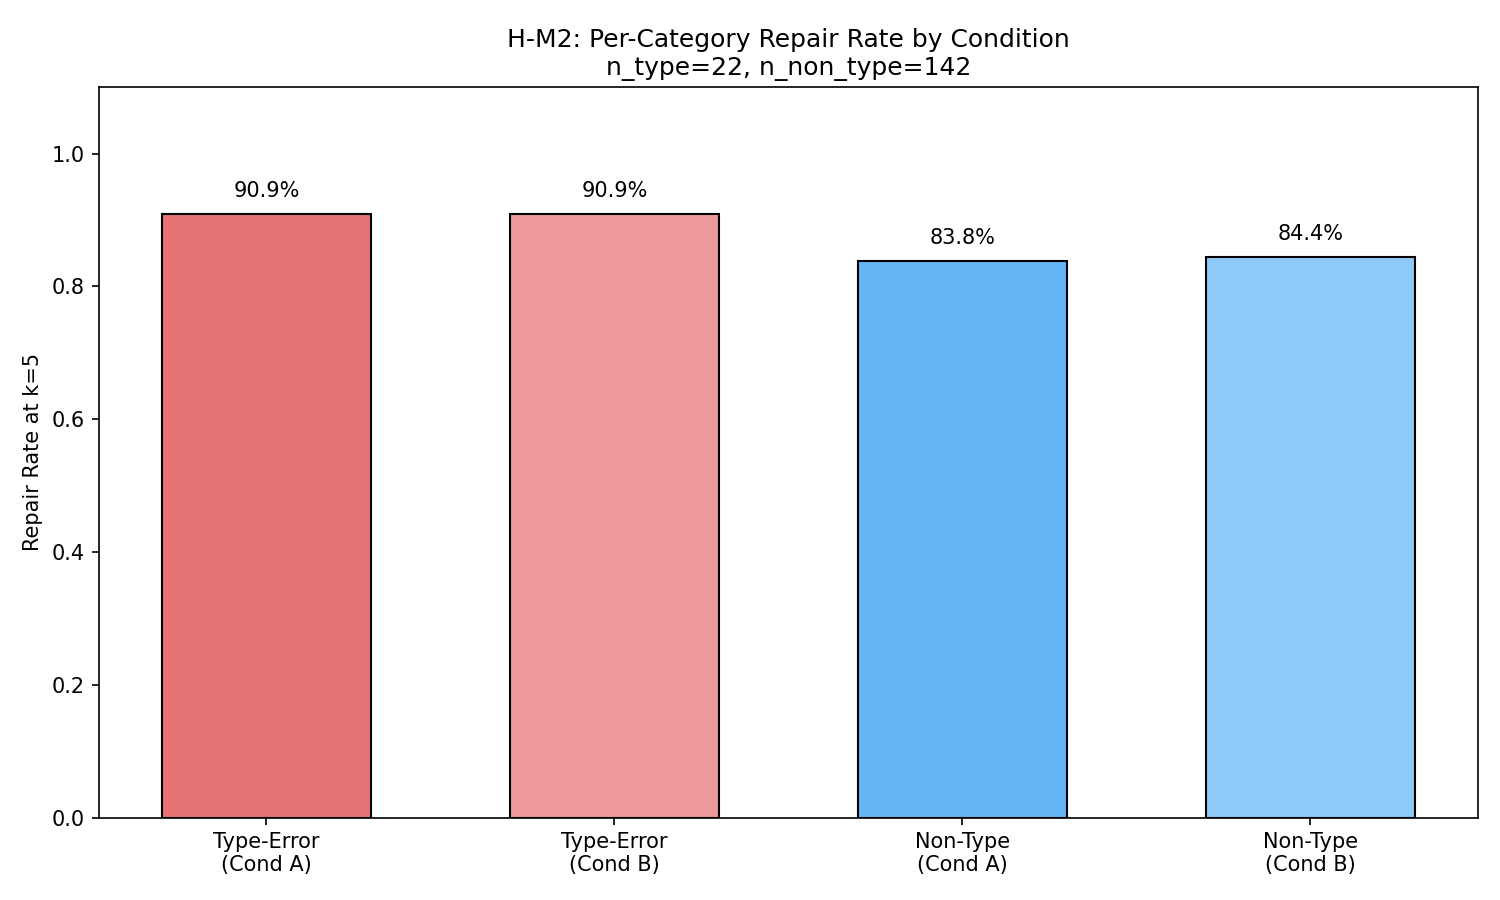
\includegraphics[width=\columnwidth]{figures/repair_rate_comparison.png}
\caption{Repair rates for type-error and non-type-error problems under Conditions A and B}
\label{fig:repair_rate_comparison}
\end{figure}

\textit{Figure 5: Repair rates (fraction of problems passing after k=5 rounds) for type-error (n=22) and non-type-error (n=142) problems under Conditions A and B. Both conditions achieve identical 90.9\% on type-error problems.}

\begin{figure}[htbp]
\centering
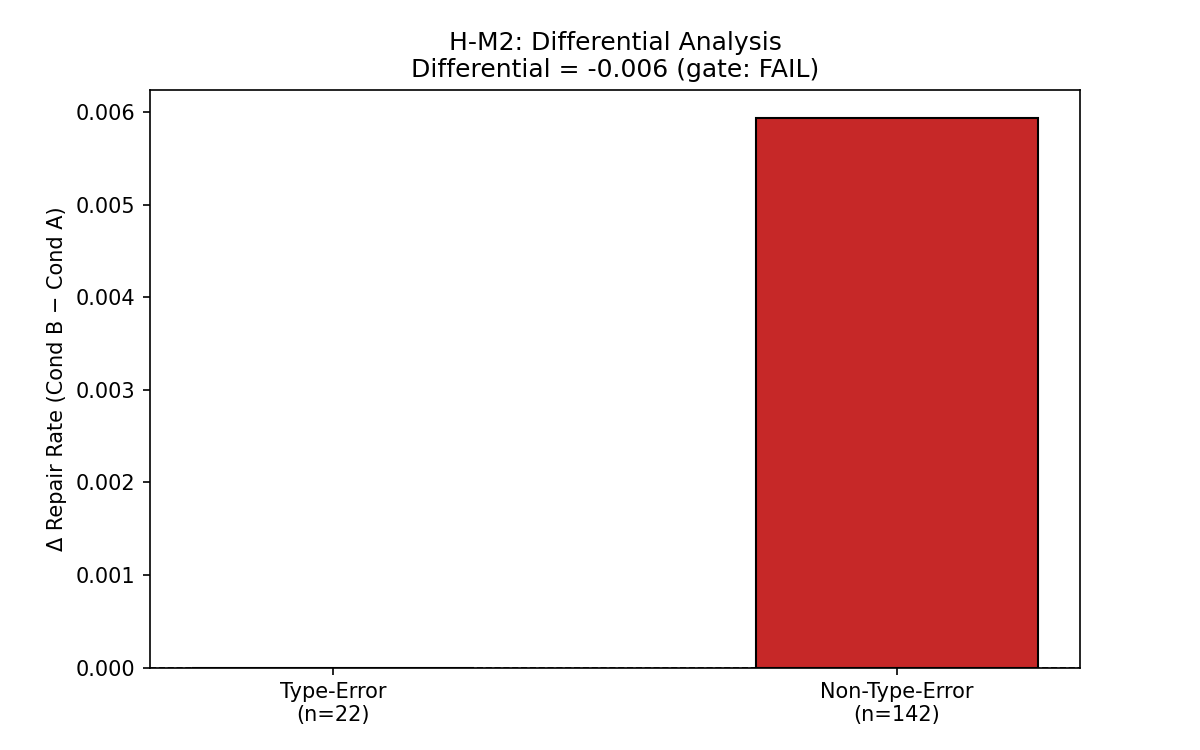
\includegraphics[width=\columnwidth]{figures/differential_chart.png}
\caption{Type-specificity differential chart}
\label{fig:differential_chart}
\end{figure}

\textit{Figure 6: Type-specificity differential (delta\_type $-$ delta\_non). Positive value would indicate type-specific benefit; observed value is $-0.006$.}

\subsubsection{RQ4: Overall Pass@1 Comparison (h-m3)}

\textbf{Table 2:} pass@1 on HumanEval+ (164 problems, GPT-4o-mini, k=5 repair rounds).

\begin{table}[htbp]
\centering
\resizebox{\columnwidth}{!}{%
\begin{tabular}{llll}
\toprule
Seed & Condition A (exec-only) & Condition B (exec+mypy) & Delta \\
\midrule
42 & 79.9\% & 86.6\% & +6.7pp \\
123 & 76.8\% & 87.8\% & +11.0pp \\
456 & 78.1\% & 87.2\% & +9.2pp \\
**Mean** & **78.25\%** & **87.20\%** & **+8.94pp** \\
\bottomrule
\end{tabular}
}
\end{table}

Seed standard deviation: Condition A = $\pm 1.56pp$; Condition B = $\pm 0.49pp$. Delta range: 6.7pp to 11.0pp.

Execution+mypy repair achieves \textbf{87.20\% pass@1} versus \textbf{78.25\%} for execution-only --- a \textbf{+8.94pp} improvement. The direction is consistent across all three seeds; no seed shows Condition A $\geq$ Condition B.

Gate h-m3 (MUST\_WORK): \textbf{PASS} --- pass@1\_B > pass@1\_A on HumanEval+ across all three seeds. Note: MBPP+ pass@1 comparison was not completed (122/378 tasks, seed=42, Condition A only); all quantitative pass@1 claims are HumanEval+-specific (see limitation L1, Section 6).

\subsubsection{RQ5: Z3 Counterexample Feedback (h-z1)}

\textbf{Table 3:} pass@1 on arithmetic subset (n=112 problems with valid Z3 specs, seed=42, k=5 repair rounds).

\begin{table}[htbp]
\centering
\resizebox{\columnwidth}{!}{%
\begin{tabular}{ll}
\toprule
Condition & pass@1 \\
\midrule
B (execution+mypy) & 86.6\% (97/112) \\
C (execution+mypy+Z3) & 85.7\% (96/112) \\
Delta (C $-$ B) & **$-0.9pp$** \\
\bottomrule
\end{tabular}
}
\end{table}

Z3 pipeline funnel: 164 HumanEval+ problems $\rightarrow$ 123 arithmetic-curated (75.0\%) $\rightarrow$ 112 valid Z3 specs (91.1\% of curated). Z3 counterexamples found in 18/112 problems (16.1\% CE activation rate). Mean CEs per problem: 0.65; maximum: 5.

Condition C does not outperform Condition B. Two factors constrain the result: (1) the CE signal activates in only 16.1\% of problems, leaving 83.9\% of Condition C problems with identical feedback to Condition B; (2) base pass@1\_B = 86.6\% leaves 13.4\% headroom for improvement, limiting the maximum observable benefit.

Gate h-z1 (SHOULD\_WORK): \textbf{FAIL} --- delta $C-B = -0.9pp \leq$ 0; limitation recorded.

\begin{figure}[htbp]
\centering
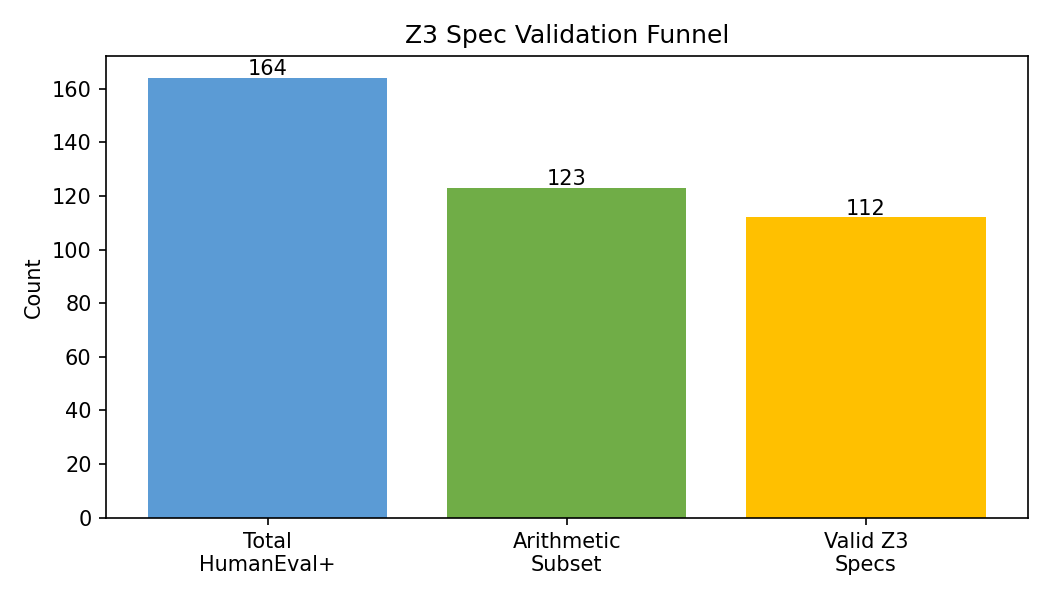
\includegraphics[width=\columnwidth]{figures/z3_funnel.png}
\caption{Z3 validation funnel}
\label{fig:z3_funnel}
\end{figure}

\textit{Figure 7: Z3 validation funnel: 123 arithmetic-curated problems $\rightarrow$ 112 valid Z3 specs (91.1\%) $\rightarrow$ 18 problems with CE found (16.1\% CE rate).}

\begin{figure}[htbp]
\centering
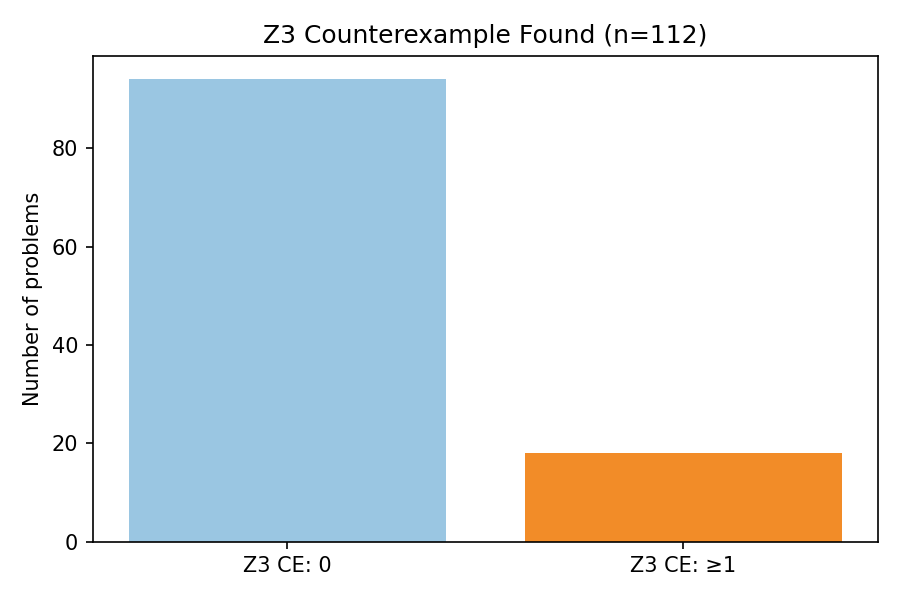
\includegraphics[width=\columnwidth]{figures/z3_ce_distribution.png}
\caption{Z3 CE found vs. not found distribution}
\label{fig:z3_ce_distribution}
\end{figure}

\textit{Figure 8: Distribution of Z3 counterexample found (18/112) versus not found (94/112) across the arithmetic subset.}

\begin{figure}[htbp]
\centering
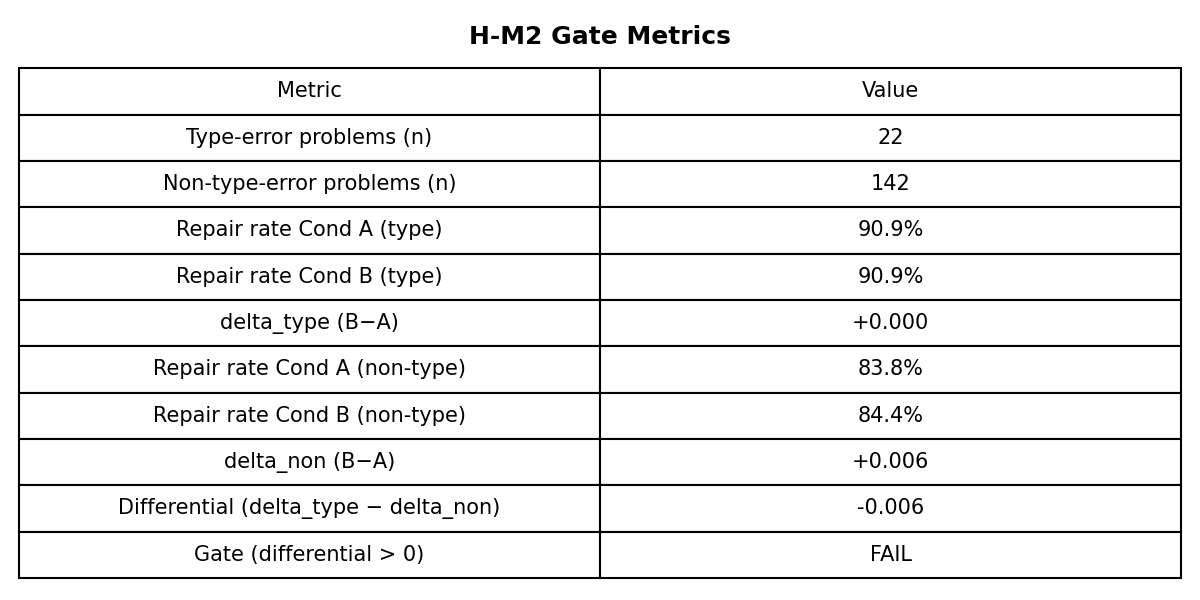
\includegraphics[width=\columnwidth]{figures/gate_metrics.png}
\caption{pass@1 comparison Condition B vs Condition C}
\label{fig:gate_metrics}
\end{figure}

\textit{Figure 9: pass@1 for Condition B (86.6\%) and Condition C (85.7\%) on the arithmetic subset (n=112). Delta = $-0.9pp$.}

\begin{figure}[htbp]
\centering
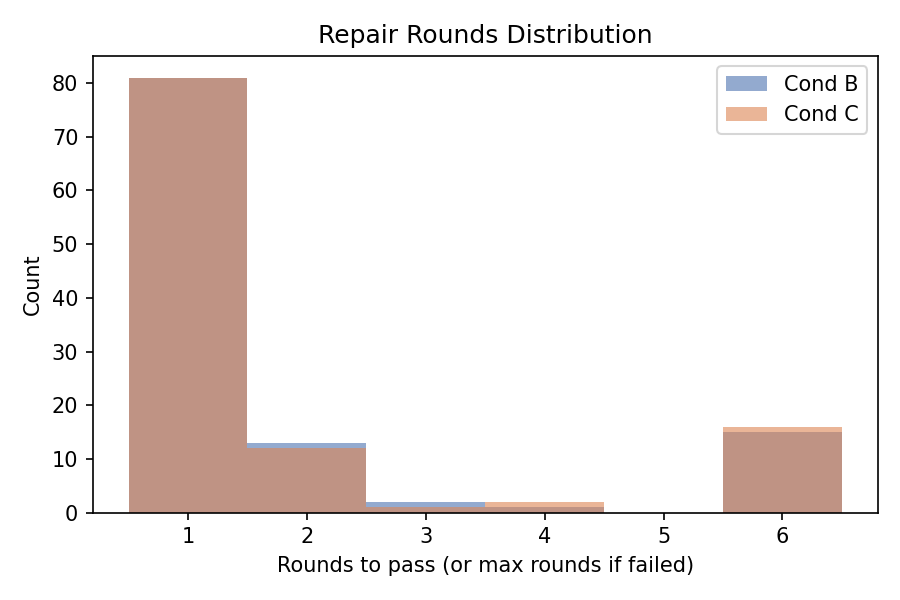
\includegraphics[width=\columnwidth]{figures/repair_rounds.png}
\caption{Repair round distribution}
\label{fig:repair_rounds}
\end{figure}

\textit{Figure 10: Repair round distribution for Conditions B and C on the arithmetic subset.}

\subsubsection{Summary}

\begin{table}[htbp]
\centering
\resizebox{\columnwidth}{!}{%
\begin{tabular}{llll}
\toprule
RQ & Sub-hypothesis & Key Finding & Gate \\
\midrule
RQ1 & h-e1 & 70\% mypy error rate on HumanEval+; 0\% on MBPP+ & PASS (MUST\_WORK) \\
RQ2 & h-m1 & Errors 1.$55\rightarrow 0.00$ by round 2; Spearman $\rho=-0.707$ & PASS (MUST\_WORK) \\
RQ3 & h-m2 & Type-specificity differential=$-0.006$; mechanism null at k=5 & FAIL (SHOULD\_WORK) \\
RQ4 & h-m3 & +8.94pp pass@1, three seeds consistent (HumanEval+ only) & PASS (MUST\_WORK) \\
RQ5 & h-z1 & $-0.9pp$; CE rate=16.1\%; ceiling at 86.6\% & FAIL (SHOULD\_WORK) \\
\bottomrule
\end{tabular}
}
\end{table}

